\documentclass[UTF8, xcolor=table]{beamer} 
\usepackage[BoldFont,SlantFont]{xeCJK} %使用中文
\setCJKmainfont[BoldFont={SimHei},ItalicFont={KaiTi}]{SimSun} 
\setCJKsansfont{SimHei} 
\setCJKfamilyfont{nwpulogo}{nwpulogo.ttf}     	% 含"西北工业大学"logo字体 
\usepackage{latexsym,amssymb,amsmath,amsbsy,amsopn,amstext,xcolor,multicol}
\usepackage{graphicx,wrapfig,fancybox}
\usepackage{float}
\usepackage{pgf,pgfarrows,pgfnodes,pgfautomata,pgfheaps,pgfshade}
\usepackage{nwpubeamer}
\usepackage[backend=bibtex,sorting=none]{biblatex} 
\usepackage{array} 
\usepackage{bm} 
\usepackage{caption} 
\usepackage[caption=false,font=scriptsize]{subfig}

\usepackage{multirow}
\usepackage{booktabs}
\usepackage{tikz}
\usepackage{tikzscale}
\usepackage{animate}
\usepackage{amsfonts}
\usepackage{amsmath,amssymb}
\usepackage{systeme,mathtools}
\usepackage{verbatim}
\definecolor{npu-blue}{RGB}{35, 104, 177}
\definecolor{npu-blue-gray}{RGB}{229, 237, 246}

\defbibheading{bibliography}[\bibname]{} %avoid printbibliography 自动生成目录
\addbibresource{ref/papers-bib-in-google.bib}
\addbibresource{ref/chinese-ref.bib}
\setbeamertemplate{bibliography item}[text] % [ref](http://tex.stackexchange.com/questions/68080/beamer-bibliography-icon)
\usepackage{boxedminipage} %for: bvh border
\def\fourgraphicswidth{0.35} %0.3\textwidth

\usepackage{algorithm} %%format of the algorithm
\usepackage{algpseudocode}
\floatname{algorithm}{算法}
\renewcommand{\algorithmicrequire}{\textbf{输入:}} %%Use Input in the format of Algorithm
\renewcommand{\algorithmicensure}{\textbf{输出:}} %%UseOutput in the format of Algorithm
%\algrenewcommand{\algorithmiccomment}[1]{\hskip3em $\rightarrow$ #1}
\algrenewcommand{\algorithmiccomment}[1]{ $//$ #1}

\usepackage{listings}
\renewcommand\lstlistingname{代码}
\renewcommand\lstlistlistingname{代码}

\lstset{framexleftmargin=1.4em,
        xleftmargin=1.8em,
        basicstyle=\ttfamily\small,
        %frame=shadowbox, numberstyle=\tiny, breaklines=true,
        frame=single,
        numberstyle=\tiny, breaklines=true,
        keywordstyle=\color{npu-blue}\bfseries,
        %commentstyle=\color{red!50!green!50!blue!50},
        rulesepcolor=\color{npu-blue-gray},
        numbers=none,fontadjust=true}
\lstdefinelanguage{shader}{morekeywords={uniform, layout, uniform, vec2, vec3, vec4, in, out, gl_Position, dot, flat, int ,float, gl_VertexID, xyz, w, x, y, z, location, version, sampler2DRect, bgr, gl_FragData, texture2DRect, gl_TexCoord,for,xy},morecomment=[l]{//}}


\begin{document}

\setbeamerfont{footnote}{size=\tiny}
\setbeamerfont{caption}{size=\scriptsize}
\setbeamertemplate{caption}[numbered]
\setbeamerfont{subsection in toc}{size=\footnotesize}
\renewcommand*{\bibfont}{\footnotesize}
\graphicspath{{figures/}}


\title{\textbf{图像去雾算法分析}}
\author[敖冠舒~叶昊宇]{
  《数学欣赏》课程报告
  \vskip 20pt 电子信息学院~敖冠舒
  \vskip 5pt 数学与统计学院~叶昊宇
  \vskip 20pt \textbf{指导教师:张胜贵~教授}}
\institute{\small \vskip 50pt西北工业大学}
\date[\today]{\small \vskip -17pt \today}
 

%校徽
\frame{
\vspace{-15mm}
\titlepage
\vspace{-43mm}
\centering
\begin{figure}[!]
    \begin{minipage}[c]{2cm}  
    \resizebox{!}{1cm}{%
    \parbox{0.54cm}{
\definecolor{npu-blue}{RGB}{35, 104, 177}
\definecolor{npu-blue-gray}{RGB}{229, 237, 246}

\setCJKfamilyfont{nwpulogo}{nwpulogo.ttf}     	% 含"西北工业大学"logo字体 
\newcommand{\nwpulogo}{\CJKfamily{nwpulogo}}
\begin{tikzpicture}
  \draw[npu-blue][line width=0.1cm] (0,0) circle (2cm);
  \draw[npu-blue][line width=0.05cm] (0,0) circle (1.3cm);
  \fill[npu-blue-gray] (0,0) circle (1.3cm);
  \fill[white] (0,0) circle (0.9cm);
  \draw[npu-blue][line width=0.05cm] (0,0) circle (0.9cm);
  \fill[npu-blue] (-0.5,-0.73) .. controls (-0.35,-0.81) ..
	(-0.2,-0.8)  .. controls (0.15, -0.7) and (0.20,-0.60) .. 
	(0.35,-0.35)   .. controls (0.42, -0.24) and (0.6,-0.26) ..
	(0.6,-0.4)   .. controls (0.58,-0.50) and (0.49, -0.50) ..
	(0.45,-0.45) .. controls (0.4,-0.68) and (0.75, -0.7) ..
	(0.9,0) arc (360:250:0.9cm);
  \fill[npu-blue] (-0.4,-0.4)--(-1.33,-0.4)--(1,1.1)--cycle;
  \fill[npu-blue] (-0.37,-0.43)--(-0.2,-0.8)--(1.01,1.05)--cycle;
  
  \foreach \x/\txt in {0/N,1/O,2/R,3/T,4/H,5/W,6/E,7/S,8/T,9/E,10/R,11/N,12/~,13/P,14/O,15/L,16/Y,17/T,18/E,19/C,20/H,21/N,22/I,23/C,24/A,25/L,26/~,27/U,28/N,29/I,30/V,31/E,32/R,33/S,34/I,35/T,36/Y}
  {
    \node[npu-blue][scale=0.7,rotate=\x*-6.5-245] at (207+\x*-6.5:1.6cm) {\txt};
  };
  \foreach \x/\txt in {0/西,1/北,2/工,3/业,4/大,5/学}
  {
    \node[npu-blue][scale=1.25,rotate=\x*18-50] at (225+\x*18:1.65cm) {\nwpulogo\txt};
  };
  \foreach \x/\txt in {0/1,1/9,2/3,3/8}
  {
    \node[npu-blue][scale=1,rotate=\x*18-25] at (\x*18-115:1.1cm) {\bfseries\txt};
  };

  % \node[npu-blue][scale=8]at (12.5,0.5){\nwpulogo 西北工业大学};
  
  % \node[npu-blue][scale=1.8]at (12.5,-1.5){NORTHWESTERN POLYTECHNICAL UNIVERSITY};
\end{tikzpicture}


}
    }
    \end{minipage}
  \end{figure}
}


  \section*{目录}
  \frame {
    \frametitle{\secname}
    \tableofcontents
  }

  \AtBeginSubsection[] %目录页不计算页码
  {
  \frame<handout:0>  
  {
  \frametitle{目录}
  \tableofcontents[current,currentsubsection]
  }
    \addtocounter{framenumber}{-1}  %目录页不计算页码
  }

  
    \section{引言}

    \subsection{概述}
    \begin{frame}
      \frametitle{概述}
      \begin{itemize}
        \item 图像去雾是一类非常有意义的图像处理问题,它的目标是恢复被雾气遮挡的图像;
        \item 图像去雾的应用场景有很多,比如:交通监控、自动驾驶、遥感观测等;
        \item 图像去雾的算法有很多,这里只介绍基于图像增强、基于物理模型、基于深度学习的三种方法。
      \end{itemize}
    \end{frame}

    \begin{frame}
      \frametitle{概述}
      \begin{figure}
        \centering
        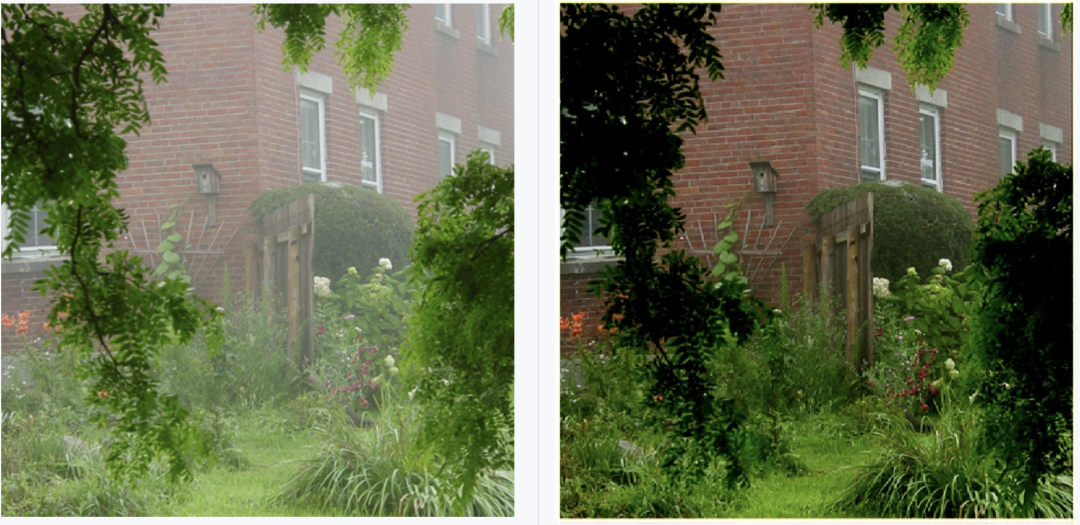
\includegraphics[width=\textwidth]{figures/pic1.png}
        \caption{图像去雾实例}
      \end{figure}
    \end{frame}

    \subsection{算法难点}
    \begin{frame}
      \frametitle{算法难点}
      \begin{itemize}
        \item \textbf{雾图特征有限}: 有雾图像由于受到雾气成像环境的干扰,其亮度、纹理、轮廓、形状等特征都存在不同程度的损失。
        \item \textbf{实时处理问题}: 如果雾图增强或复原花费的计算或存储开销过大,势必极大影响应用系统的实时工作。
        \item \textbf{普适性问题}: 算法面临的最大问题是对不同类型的雾图难以获得一致的增强或复原质量。
      \end{itemize}
    \end{frame}




  
    \section{基于图像增强}

    \subsection{直方图均衡化}
    \begin{frame}
      \frametitle{直方图均衡化}
      直方图均衡化算法的基本思想是通过直方图均衡化来扩大原有雾图像的灰度范围,改善原有雾图像对比度低的问题。
      \begin{figure}
        \centering
        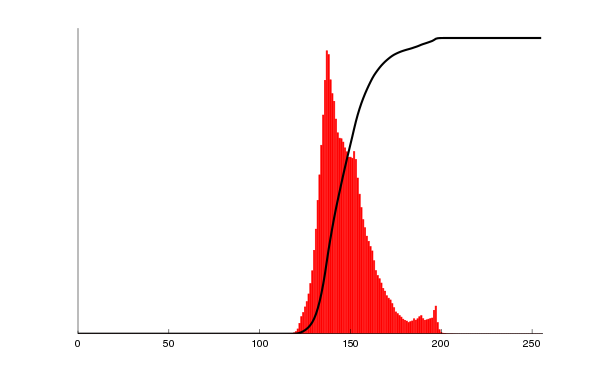
\includegraphics[width=0.47\textwidth]{figures/pic2.png}
        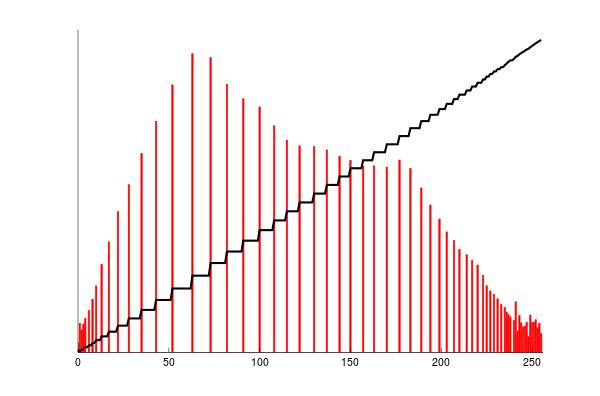
\includegraphics[width=0.45\textwidth]{figures/pic3.png}
        \caption{直方图均衡化示意图}
      \end{figure}
    \end{frame}
    \begin{frame}
      \frametitle{直方图均衡化}
      \begin{figure}
        \centering
        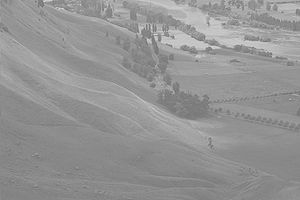
\includegraphics[width=0.45\textwidth]{figures/pic4.jpg}
        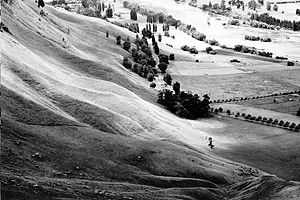
\includegraphics[width=0.45\textwidth]{figures/pic5.jpg}
        \caption{直方图均衡化效果图}
      \end{figure}
    \end{frame}


    \subsection{同态滤波}
    \begin{frame}
      \frametitle{同态滤波}
      同态滤波是一种在频域内对图像进行对比度增强的算法。同态滤波算法将有雾图像的复原问题转换成增大有雾图像频域范围的问题,通过减少有雾图像中的低频信息,并相应增加图像中的高频信息,可以实现图像去雾的效果。
      \begin{figure}%插入一张图片
        \centering
        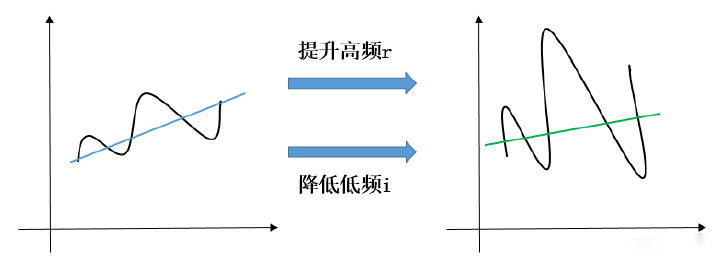
\includegraphics[width=\textwidth]{figures/pic6.png}
        \caption{同态滤波示意图}
      \end{figure}
    \end{frame}

    \begin{frame}
      \begin{equation}
        f(x,y)=i(x,y)·r(x,y)
      \end{equation}

      \begin{equation}
        z(x,y)=\ln f(x,y) =\ln i(x,y) +\ln r(x,y)
      \end{equation}

      \begin{equation}
        Z(u,v)=Fi(u,v) +Fr(u,v)
      \end{equation}

      \begin{equation}
        S(u,v)=H(u,v)S(u,v)=H(u,v)·Fi(u,v) +H(u,v)·Fr(u,v)
      \end{equation}

      \begin{equation}
        s(u,v)=IDFT(S(u,v))
      \end{equation}

      \begin{equation}
        g(x,y)=e^{s(x,y)}=io(x,y)·ro(x,y)
      \end{equation}
    \end{frame}


    \begin{frame}
      \frametitle{同态滤波}
      \begin{figure}%插入一张图片
        \centering
        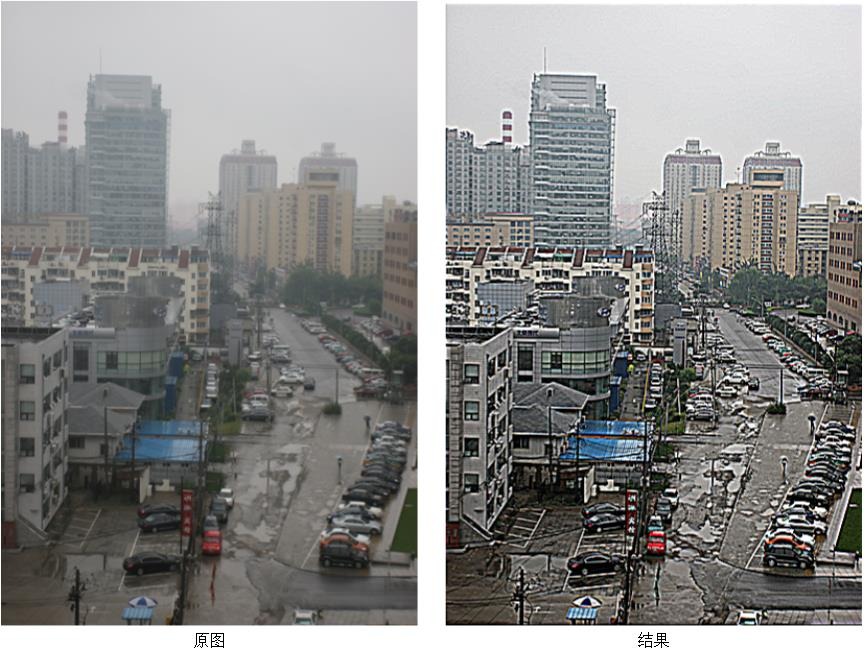
\includegraphics[width=0.8\textwidth]{figures/pic7.png}
        \caption{同态滤波效果图}
      \end{figure}
    \end{frame}


    \subsection{Retinex算法}
    \begin{frame}
      \frametitle{Retinex算法}
      Retinex算法是一种基于人类视觉系统的图像增强算法,它通过对图像进行多尺度分解,然后对每个尺度的图像进行对比度增强,最后将所有尺度的图像进行融合,从而实现图像增强的目的。

      \centering
      %斜体字
      \textit{Retinex~=~retina(视网膜)~+~cortex(皮层)}

    \end{frame}

    \begin{frame}
      \frametitle{Retinex算法}
      \begin{itemize}
        \item 1.将一幅有雾图像$S(x,y)$表示成反射分量$R(x,y)$和亮度分量$L(x,y)$的乘积形式:
          \begin{equation}
            S(x,y)=R(x,y)·L(x,y)
          \end{equation}
        \item 2.对第一步中的式两边分别取对数并移项,结果如下:
          \begin{equation}
            \ln(R(x,y))=\ln(S(x,y))-\ln(L(x,y))
          \end{equation}
      \end{itemize}
    \end{frame}

    \begin{frame}
      \frametitle{Retinex算法}
      \begin{itemize}
        \item 3.对上式去除亮度分量$L(x, y)$,求得反射分量 $R(u, v)$,从而得到增强后的图像,实现原图像的去雾处理。
        \begin{equation}
              L(x,y)=S(x,y)*H(x,y)
        \end{equation}
        \begin{equation}
              H(x,y)=u·exp(-\frac{x^2+y^2}{\sigma^2})
        \end{equation}

        $*$为卷积操作,$u$为归一化值,$\sigma$为高斯环绕尺度参数。
        \begin{equation}
           \ln(R_c(x,y))=\ln(S_c(x,y))-\ln(S_c(x,y) * H(x,y))
        \end{equation}

        $c$表示彩色图像RGB颜色空间中的某一颜色通道。

      \end{itemize}
    \end{frame}


  
    \section{基于物理模型}

    \subsection{暗通道先验}

    \begin{frame}
      \frametitle{大气散射模型}
      \begin{figure}
        \centering
        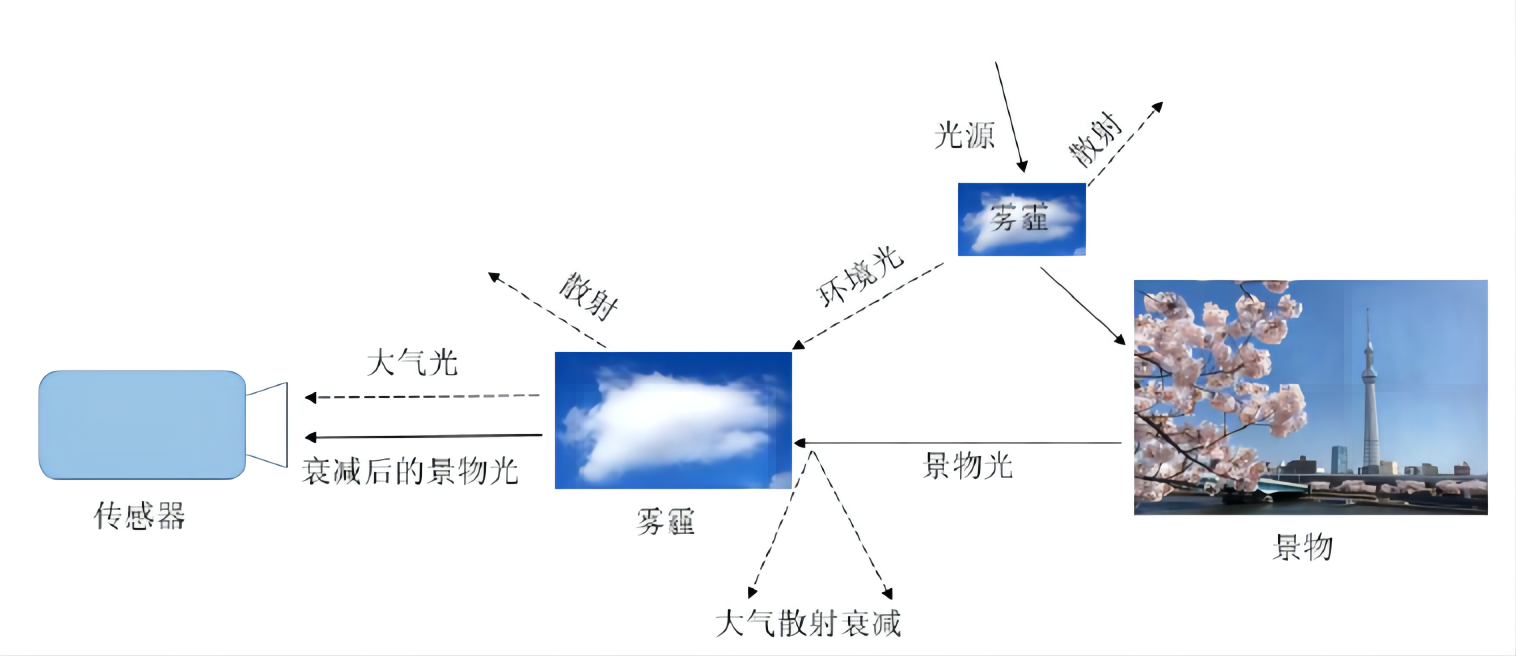
\includegraphics[width=\textwidth]{figures/pic8.png}
        \caption{大气散射模型示意图}
      \end{figure}
    \end{frame}

    \begin{frame}
      \frametitle{暗通道先验}
      对于一幅彩色图像在绝大多数非天空的局部区域里,某一些像素总会有至少一个颜色通道具有很低的值。换言之,该区域光强度的最小值是个很小的数。暗通道的数学定义为对于任意的输入图像$J$,其暗通道可以用下式表达:
      \begin{equation}
        J^{dark}(x)=\min _{y \in \Omega(x)}\left(\min _{c \in(r, g, b)} J^{c}(y)\right)
      \end{equation}
      其中,$J^c$为清晰图像$J(x)$三种色彩通道,$\Omega(x)$为图像$J(x)$中以像素$x$为中心的某一窗口,窗口大小可以根据实际情况适当调整。上式意思为:一个暗通道的值等于取一个局部窗口中每个像素点三个通道中最小值组成的集合的最小值。通过对整幅图像进行上面的操作便可以得到一幅暗通道图。
    
    \end{frame}

    \begin{frame}
      \frametitle{暗通道先验}
      作者通过大量的统计得到的先验理论指出:
      \begin{equation}
        J^{dark} \to 0
      \end{equation}
      即对于无雾的非天空部分图像的暗通道值总是趋于 0。
        
      因此,可以通过暗通道图像的最小值来估计图像的雾度。具体的,作者提出了一种基于暗通道的雾度估计方法,其数学表达式为:
      \begin{equation}
        \hat{A}=\min _{x} J^{dark}(x)
      \end{equation}
    \end{frame}

    \begin{frame}
      \frametitle{暗通道先验}
      \begin{figure}
        \centering
        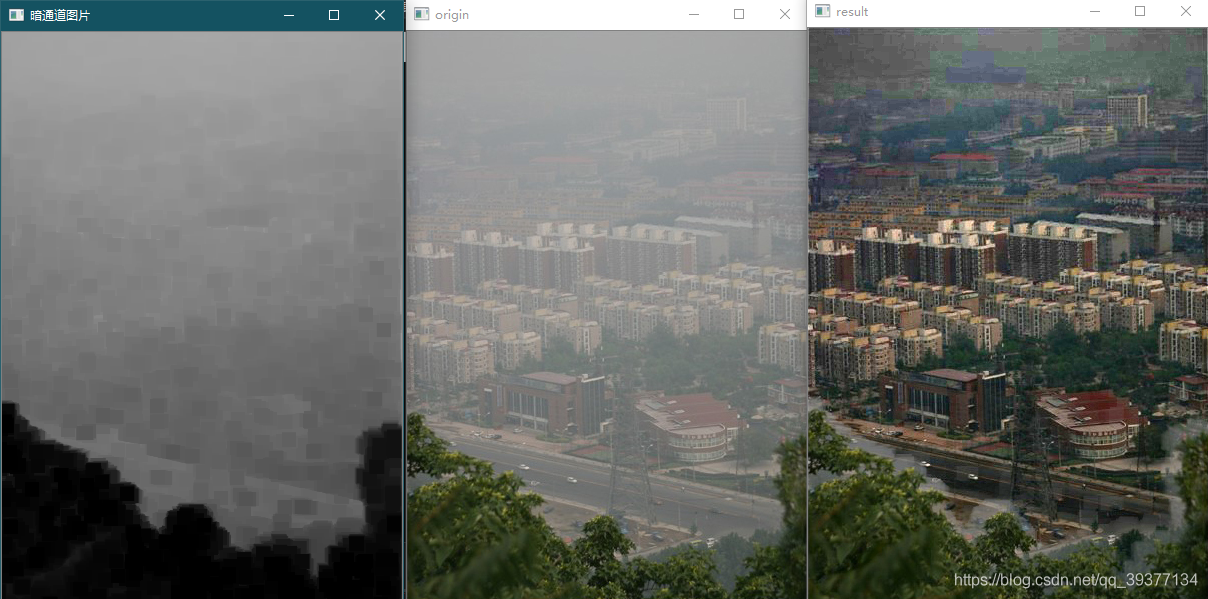
\includegraphics[width=\textwidth]{figures/pic9.png}
        \caption{暗通道先验效果图}
      \end{figure}
    \end{frame}
      \section{基于深度学习}
    
    \subsection{DehazeNet}
    \begin{frame}
    \frametitle{基于深度学习的去雾算法}
    根据深度学习模型的输出是否为去雾后的清晰图像,可以将基于深度学习的去雾算法分为两类:
    \begin{itemize}
    \item 第一类算法首先通过建立深度学习模型来估计大气散射模型中的未知参数—透射率图,再基于先验理论估计大气光照值,最后根据大气散射模型变形公式恢复对应的无雾图像,即基于非端到端的网络模型实现图像去雾
    \item 第二类算法直接建立深度学习模型恢复无雾图像,即基于端到端的网络
    模型实现图像去雾
    \end{itemize}
    \end{frame}

    \begin{frame}
      \frametitle{DehazeNet}
      \begin{figure}[h]
        \centering
        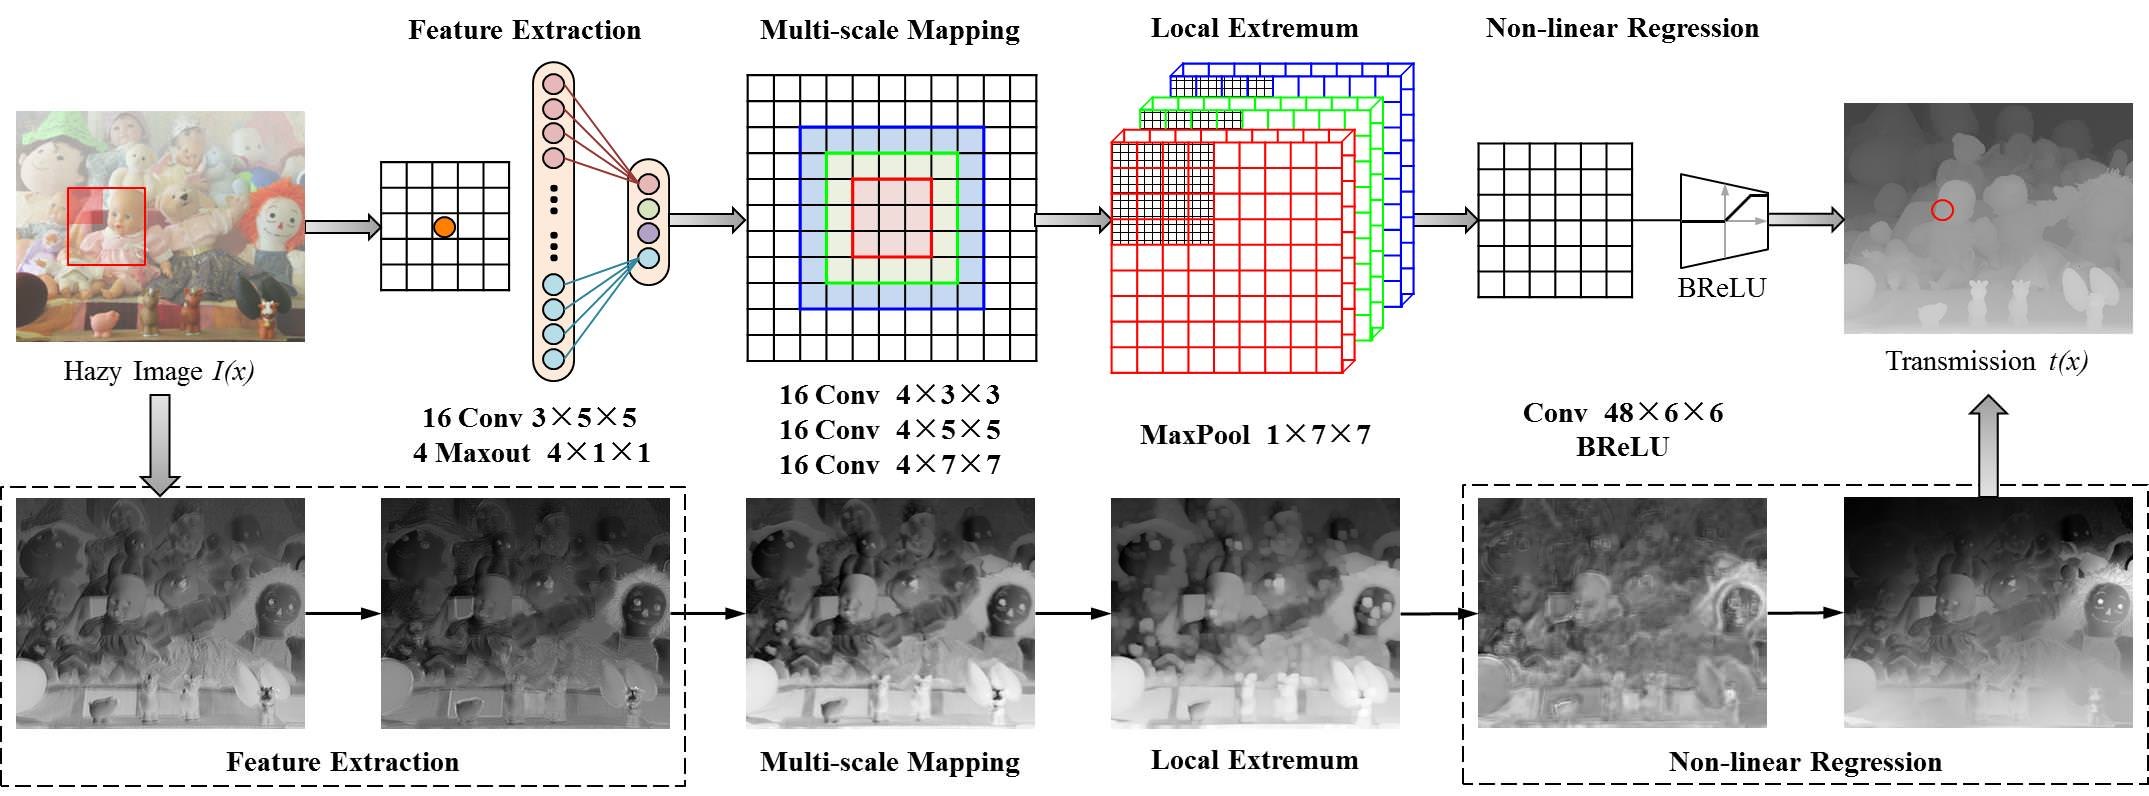
\includegraphics[width=\linewidth]{figures/pic10.png}
        \caption{DehazeNet结构示意图}
      \end{figure}
      \end{frame}

    \begin{frame}
      \frametitle{DehazeNet}
      \begin{figure}[h]
        \centering
        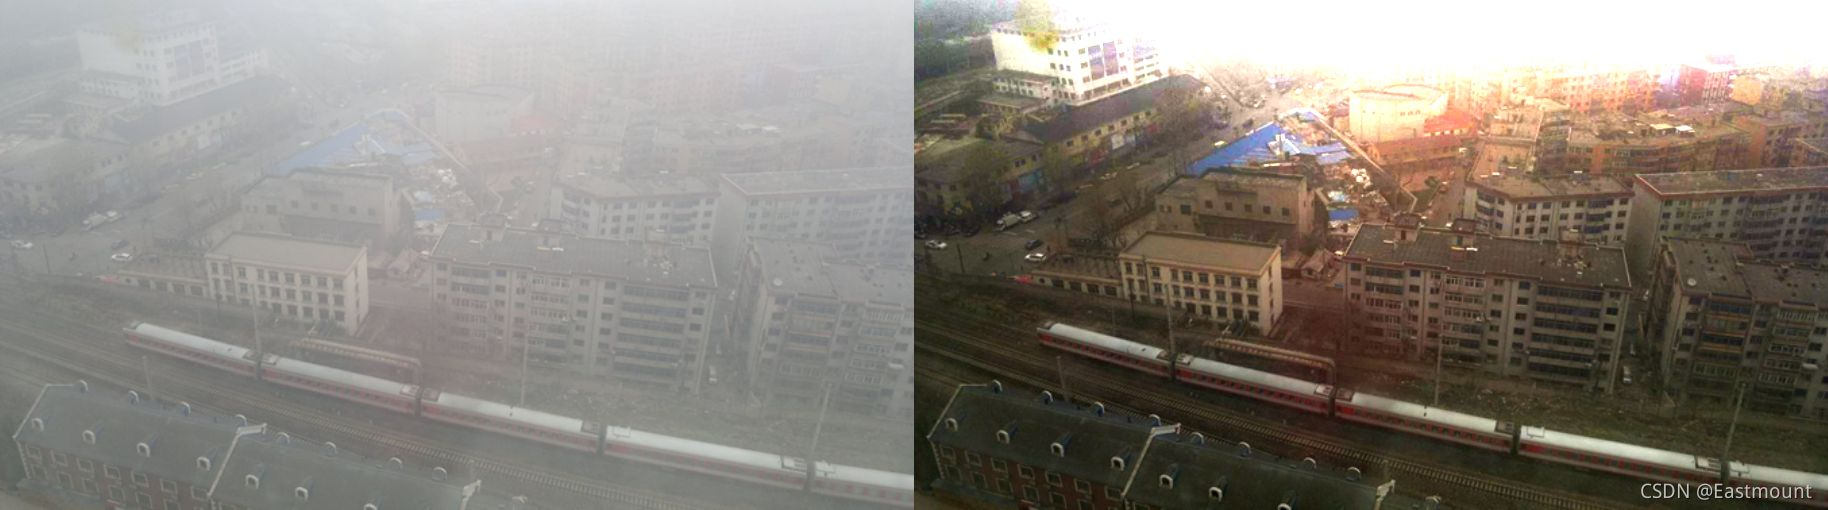
\includegraphics[width=\linewidth]{figures/pic12.jpg}
        \caption{DehazeNet去雾效果图}
      \end{figure}
    \end{frame}
  

    \subsection{AOD-Net}
    \begin{frame}
    \frametitle{AOD-Net}
    \begin{figure}[h]
      \centering
      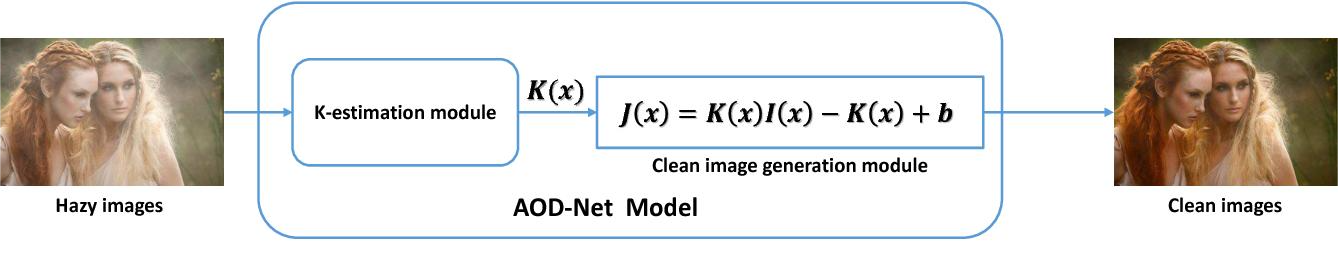
\includegraphics[width=\linewidth]{figures/pic11.png}
      \caption{AOD-Net结构示意图}
    \end{figure}
    \end{frame}

    \begin{frame}
      \frametitle{AOD-Net}
      \begin{figure}[h]
        \centering
        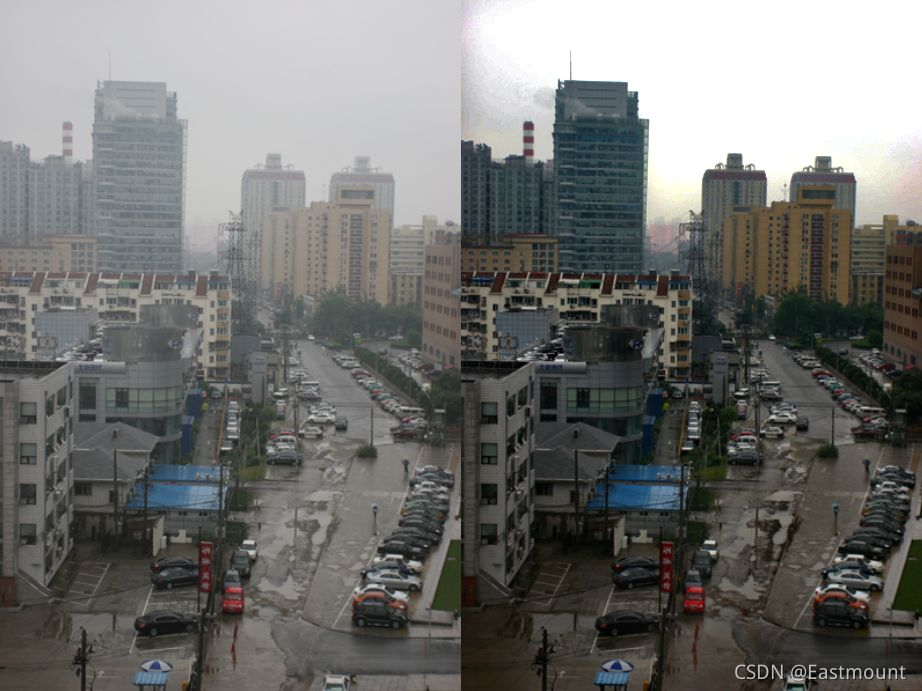
\includegraphics[width=0.8\linewidth]{figures/pic13.jpg}
        \caption{AOD-Net去雾效果图}
      \end{figure}
    \end{frame}


      \section{总结}
    \subsection{总结}

    \begin{frame}
      \frametitle{总结}
      \begin{itemize}
        \item 基于图像增强的方法不考虑有雾图像的形成过程,而是直接通过突出图像的细节,提高对比度等方式,从而使有雾图像看上去更加清晰。
        \item 基于物理模型的方法则是追寻图像降质的物理过程,通过物理模型还原出清晰的图像。
        \item 基于深度学习的方法则是利用神经网络强大的学习能力,寻找有雾图像与图像复原物理模型中某些系数的映射关系或者使用 GAN,根据有雾图像还原出无雾的清晰图像。
      \end{itemize}
    \end{frame}

    \begin{frame}
      \frametitle{总结}
      上述三类去雾算法对于雾天图像都有着明显的去雾效果,尽管其在实际生活中已经得到了广泛的应用,但下述几点仍有可能是今后图像去雾领域的研究重点和难点:
      \begin{itemize}
        \item 更加真实的雾天图像数据集
        \item 更加简便的去雾算法
        \item 鲁棒性更强的去雾算法
      \end{itemize}
    \end{frame}

    \begin{frame}
      \begin{figure}
        \centering
        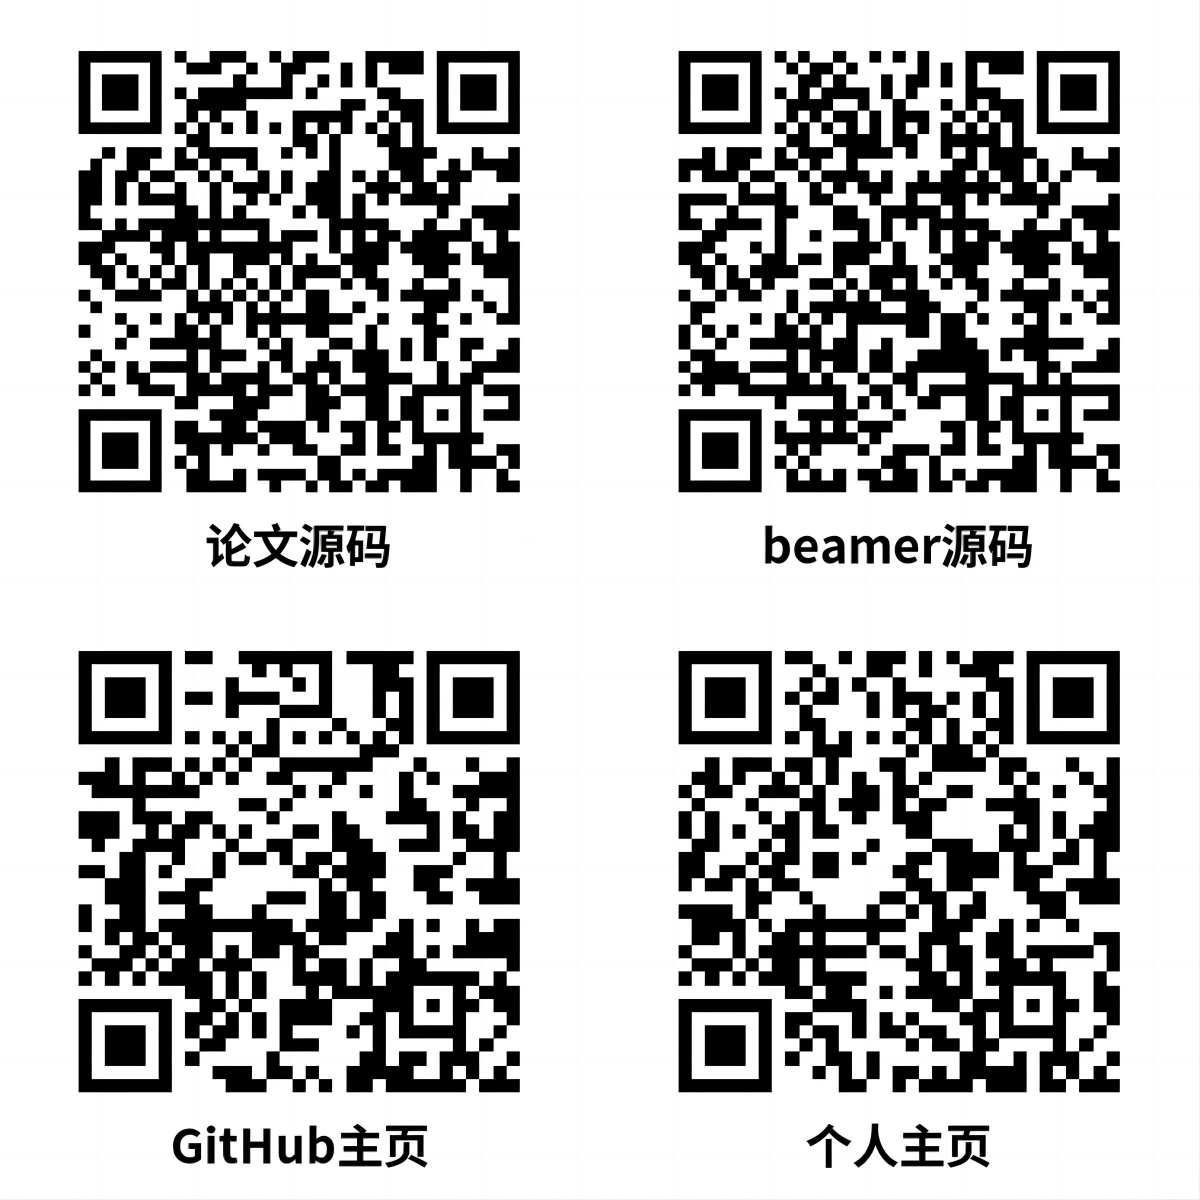
\includegraphics[width=0.7\textwidth]{figures/fusion.png}
        \caption{资源分享}
        \end{figure}
    \end{frame}


    \frame{
      \frametitle{ }
      
       ~\\ ~\\
       \center{\Large{\textbf{Thank you!}}}
       \\ ~\\ ~\\ ~\\ ~\\ 

    }

  
\end{document}

